
%LTeX: language=it
\begin{figure}[H]
    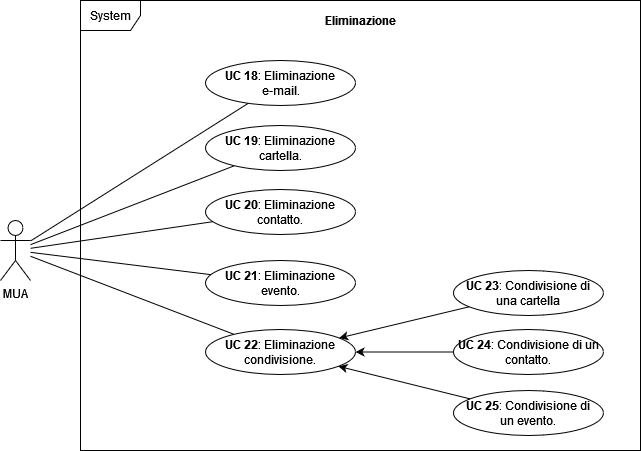
\includegraphics[width=0.75\textwidth]{sections/uc_imgs/UC-eliminazione.png}
    \centering
    \caption{Casi d'uso relativi all'eliminazione}
\end{figure}

\subsection{UC 18 - Eliminazione e-mail} \label{sec:UC18}

    \begin{itemize}
        \item \textbf{Attore principale}: MUA;
        \item \textbf{Descrizione}: il MUA deve poter eliminare un'e-mail nel sistema;
        \item \textbf{Precondizioni}: l’account che il MUA gestisce è registrato nel sistema, ha una connessione aperta con il sistema ed è autenticato;
        \item \textbf{Postcondizioni}: l'e-mail è stata eliminata con successo ed è stata rimossa dal sistema;
        \item \textbf{Scenario principale}:
            \begin{enumerate}
                \item il MUA trasmette l'id dell'e-mail da eliminare (\hyperref[sec:UC18.1]{UC 18.1});
                \item il sistema rimuove l'e-mail dal sistema.
            \end{enumerate}
        \item \textbf{Inclusioni}: nessuna;
        \item \textbf{Generalizzazioni}: nessuna;
        \item \textbf{Estensioni}: nessuna.
    \end{itemize}

    \begin{figure}[H]
        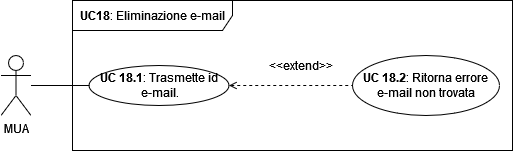
\includegraphics[width=0.75\textwidth]{sections/uc_imgs/UC18.png}
        \centering
        \caption{Diagramma sotto-casi UC 18}
    \end{figure}


\subsubsection{UC 18.1 - Trasmette id e-mail} \label{sec:UC18.1}
\begin{itemize}
    \item \textbf{Attore principale}: MUA;
    \item \textbf{Descrizione}: il MUA invia al sistema l'id dell'e-mail;
    \item \textbf{Precondizioni}: il MUA sta usando la funzionalità di eliminazione di un'e-mail;
    \item \textbf{Postcondizioni}: il sistema conosce l'id dell'e-mail da eliminare;
    \item \textbf{Scenario principale}:
        \begin{enumerate}
            \item il MUA trasmette l'id dell'e-mail;
        \end{enumerate}
    \item \textbf{Inclusioni}: nessuna;
    \item \textbf{Generalizzazioni}: nessuna;
    \item \textbf{Estensioni}:
        \begin{enumerate}[label=\alph*.]
            \item l'id dell'e-mail non è stato trovato:
            \begin{enumerate}[label=\arabic*.]
                \item il sistema ritorna un errore di e-mail non trovata (\hyperref[sec:UC18.2]{UC 18.2}).
            \end{enumerate}
        \end{enumerate}
\end{itemize}


\subsubsection{UC 18.2 - Ritorna errore e-mail non trovata} \label{sec:UC18.2}
    \begin{itemize}
        \item \textbf{Attore principale}: MUA;
        \item \textbf{Descrizione}: il sistema non riesce ad eliminare l'e-mail perché l'e-mail non è stata trovata;
        \item \textbf{Precondizioni}: il MUA ha inviato l'id dell'e-mail da eliminare;
        \item \textbf{Postcondizioni}: il sistema non elimina l'e-mail, il MUA è stato notificato dell'errore;
        \item \textbf{Scenario principale}:
            \begin{enumerate}
                \item il sistema non trova l'e-mail con l'identificativo fornito dal MUA;
                \item il sistema non elimina l'e-mail e notifica il MUA dell'errore;
            \end{enumerate}
        \item \textbf{Inclusioni}: nessuna;
        \item \textbf{Generalizzazioni}: nessuna;
        \item \textbf{Estensioni}: nessuna.
    \end{itemize}
